\documentclass[main.tex]{subfiles}

\begin{document}

\linksection{Лекция 06.12.2023 (Смольская Н.Б.)}

As I promised last week, today we shall continue practising your monologues and your speech practice, your spoken English.
And for today I think we will do it on the basis of the very first topic, from the point of view of order, and I think from the most simplest one, which is "<Мои научные интересы и моя научная деятельность">.
It is not by chance that I actually name this topic in Russian, because I would like you to think how to translate it into English.
And that will be your choice.
So, I would like to arrange this part of our class in the way that you will have again five, from five to seven minutes, not more, because the more you think, the more difficult it becomes actually to speak and to present all the information that you have.
So, I would like each of you to, at this point, not to write down the text, but again to write down the keywords or the key phrases that you would think would help you to present this topic.
But after that, I don't know, maybe we will, I don't know, I will arrange it in, I don't know, "<камень-ножницы-бумага">.
So I haven't decided yet.
I have five minutes to think how to arrange it.

So today I would like you to practise the whole task, number three, which is to present a monologue and then to answer the questions.
But the questions will be from the peers, not from me, and I will just listen to your questions because the next step or the next stage that we will practise and discuss today will be the questions -- the types of questions in the English language, which is also important.
Because when you are asked questions, you should actually know exactly what to answer, what type of question you are asked and what is required from you, from the point of view of the type of the question, because it is also important.
The English language is very pragmatic in the sense, in the aspect of asking questions.
Because if you're asked a particular type of question, it means that you should present a particular type of answer, nothing more.
Otherwise it will lead to, I hope, no grammar mistakes, but unnecessary information.
So you should answer what you are asked.
So that is why.

So we will have a very comfortable place here, so those who will be in charge of presenting a monologue will enjoy standing here.
It is very nice, it is very comfortable here, and those who will be the listeners will actually, in any case, actively participate in the discussion because while listening, I would like you, well, at least each of you to think of one question, what you would like to ask your peer colleague, your peer standing here and suffering in monologue speech, which is not difficult at all, as you understand.
So, again, I would like you not to write down the whole sentences.
I do repeat it again because I'm not interested in writing sentences.
I would like you to speak using the anchors, the anchor words that you should use when presenting the topics.
So you're welcome to spend, I think, not more than five minutes, because that's not difficult at all.
So take your time.
Five minutes to think about, that can be even a plan.
The plan in the form of the phrases, the plan in the form of the keywords.
So, "<Мои научные интересы и моя научная деятельность">.

You should actually clearly understand that is it like a sort of a generalised (a bigger) sphere and something narrower, which is within the sphere of scientific interests.
I mean, how actually you apply and implement those things that are interesting for you in some particular specific activities.
So take your time.
Five minutes, not more, for you not to start broadening the ideas.

Используем время с пользой!
\\

--- Выполнение задания ---
\\

So, ready?
I was thinking how to choose but maybe for today let it be your personal choice.
Maybe there are those who would like to practise speaking, those who are, maybe those who have skills of speaking.
May I?
Yes, you're welcome.
You see ladies first as usual, as always.
Yes, of course.
So, you listen attentively and make sure that you know and you make sure that you know what to ask.
Okay, you're welcome.

\newpage
\sublinksection{My scientific interests and my academic activity. My department}

Hello my dear colleagues, my name is Olga and I have some problems with English but I hope you will know any questions for my topic (for my monologue).
First of all, I wanted to say that I finished St.
Petersburg Technological Institute in program that connected with chemical technologies, oil refining and all that connected with it.
I like chemistry and I want to start and to continue my project, my candidate project, in this year.
Also, I finished Polytechnic University in program of medical modelling and mechanics.
And I like so much Polytechnic University and I hope it will be the best university in the whole world.
About my project.
I love chemistry and I like mathematic modelling and I want to connect it in one sphere.
My topic is connected with polymers and composites and I want to model such properties as ...
I forgot some words about my topic.
I hope you will understand me.
Sorry for it.
In general I want to model composites.
I want to model polymers.
And I hope it will save a lot of lives in the world.
And I think that's all.
Because all that I wanted to say, I forgot.
Thank you so much for attention.

So you're welcome.
If you have any questions ...
Definitely, they should.
Not because what you said is actually questionable, just because this is the task for them to ask questions and you to try to answer them.
So, gentlemen, you're welcome.
Okay, you're welcome.
Let's speak.
What types of composite materials you want to model?
It will be very difficult word in Russian and more difficult in English.
Биосовместимые.
I will see on structure of materials, I will print it on a 3D-printer and then I will use it in medical spheres.
Okay, thank you.
I don't understand why you are afraid.
Okay, so, gentlemen, no questions.
I have one question.
What are the most interesting qualities what you want to model?
What are the most interesting qualities for you to model?
I want to create new polymer and new composite that will be healthy for person and it can be used in another spheres, such as oil and gas refining.
Some kind of universal composite that can be implemented in both in some biotechnologies and other spheres?
It is me dream.
I hope it will be.
Olga, is your research about some prosthesis?
Yes, we have.
We have made in our department of Theoretical Mechanics some prosthesis of heart, of hand and...
Okay, thank you.
Could you tell me please what type of body part you want to modify with your prosthesis, I guess, or just help some people.
It is general question for me...
I think the material of your polymer depends on the type of body, part of body, where you want to implement it...
Yes of course you are right.
And I don't know what to say now but I can speak about it later in six months I think.
And we will discuss it.
Okay, so, any more questions?
So thank you Olga.
Great!
Thank you for being the first.
So gentlemen who would like now to take the floor?
You see, that's not frightening at all, because you all will have to suffer through it during your examination.
But I prefer now.
So as you see, I do not want to stop you or to interrupt you by interrupting your speech, so I just make some notes of what we should repeat when discussing grammar.
So at this point, you just speak and your colleagues ask.
So, you are welcome.

Good evening, my dear colleagues.
My scientific interest is connected with one of the biggest problems of energy.
It is about...
It's connected with emissions reductions.
One of the solutions of this problem is designing more efficient turbines, steam turbines, gas turbines.
And it leads to design more efficient turbine blades.
One of them is Longitudinal.
They are very flexible, potentially excitable.
And my thesis is modelling of forced vibration of blades.
It helps to design blades that are resistant to different excitations.
For example, flutter, torsional oscillation of prototype, and so on.
That's all.

Okay, questions, questions, make yourself ask questions, that's also nice and important and useful I would say.
Which questions? Any questions.
Important questions.
Somehow related to the theme or to the idea presented.
How modifying the turbine will reduce the emission?
If you design a more efficient blade, you design a more efficient turbine.
A more efficient turbine leads to fuel consumption reduction.
Okay.
Anything else?
I want to ask.
What software, what CAD (computer-aided engineering) software you will use during your work?
I will model blades by finite elements method in Ansys Mechanic.
Any other questions? I fixed the questions to use them during the examination.
In what area can be used these turbines?
In which area?
Yeah.
These turbines will be used in thermal or nuclear power plants.
Please tell me, I understood you correctly.
This task, this target is for your job?
Yes.
That's my profession.
What type of benefits your company will give you after you finish your job, your scientific work?
What will be the bonuses?
Money.
Just money?
Any promotion?
Okay, yes.
Promotion, respect and money.
Which parameters can be changed in your blade or turbine model?
Some material or shape parameters?
My research is about post-vibration of blades, not of design these blades.
Only calculation!
There are stress-strain states, and there are natural frequencies, natural moves.
Thank you.
Okay.
Anything else? Thank you very much.
So you see sometimes it is even interesting to present your interests in English because the discussion is very active.
So who else would like to practise?
You are welcome.
Because you can have a feedback to your interests.

So it is very useful for me because my supervisor will force me to speak in English.
So, hello, my name is Nikita.
I graduated from Peter the Great University from Building Engineering Institute, yes.
And that's why my scientific interests are connected with buildings and civil engineering.
There is mechanical engineering, material science, also BIM-technologies are very interesting for me.
And of course, building structures.
So my project, my scientific work, is about intermodal connections of module buildings.
I think where is steel in buildings.
And this work is aimed to develop this sphere and model buildings at all and in Russia because there are some problems in this area and one of the biggest problem is that there are no norms and calculations.
And I want to create quite simple analytical calculation methods for designing and testing the intermodal connections without using ANSYS.
I will use ANSYS in my work, but I want to make method without using ANSYS or such complex programs.
I think that's all.

Okay, thank you.
Questions?
Nikita, you said that you will be modelling steel constructions?
Are you looking to model complex constructions?
I don't know exactly.
Maybe I will try also to model complex polymer materials but I will start with steel construction and steel connections.
Okay.
So, anyone else?
Пользуйтесь возможностью задать вопрос.
Nikita, as I understood you will try to create some package or application where, for example, a user like me or you can, to enter some parameters of your, for example, building, and give some properties of your solution.
Not exactly, but this is very nice idea to create some soft.
In the basic idea it is analytical method, it is formula, such as regulations, such as regulation 63.
And it will be connected only with intermodal connections.
So you have to know the forces and you can design this connection (maybe welded, maybe with bolts) and calculate the thickness of plates.
I asked because you said that you don't want to use any programs like ANSYS or other programs.
So, as for user, what's our benefit?
Maybe I told it incorrect.
I will use these programs to verify.
To verify, yes.
But just for users...
What do you want to give, for example, for user experience maybe, or any features?
I want to give this method.
Using this method you can design or test connection or type of connection.
Because now there isn't any methods not using ANSYS or ABAQUS in construction.
Thank you.
Nikita, you said that you may model a polymer in your research.
Is it about some self-repairing concrete?
No, I thought about complex polymer material, it is fiberglass or fiberbaselts.
I know that your adviser is a head of laboratory of self-repaired materials.
Yes, now I don't aim to use and calculate concrete, maybe in the future researches.
Thank you very much.
So one more person and we continue.
So who would like to? Thank you very much.
Я надеюсь, что остальные тоже будут дальше заставлять себя, хотя бы вопросы задавать.

First of all I will try to answer the question that Maxime asked.
I mean, in constructions, people don't use such specific programs like Abaqus and Ansys to do calculations.
These people always try to use regulations and expressions.
So it's important that all solutions was been written in regulations.
And my situation is something similar.
I want to do research in modular construction, but it's consistent with nuclear waste.
They usually stored in specific containers and in the nuclear storage these containers are usually stacked.
It's important to define the seismic resistance.
And also in this case there are no expression and regulations how to do it.
So my work is consist to analyze what type of oscillations will occur and maybe trying to obtain some simple solutions and trying to create the method to define the maximum amplitudes in selections.

Okay, so you see how many words and how many terminological words I would say, you know.
For me, there is a great number of words that I do not even understand.
Not even know to understand.
Okay, so, you're welcome.
Questions? Not maybe specific, something general, not a general question, sorry, because there is no...
Yes, you are welcome.
You said that construction solutions are based only on regulations, for example, but as I know, in this sphere we can see, for example, use these methods from "<строймех"> to build constructions or create some buildings, make some prototypes, for example.
I don't understand your question.
You told that construction, building engineers, construction engineers, I don't know how it's.
Civil engineers.
Civil engineers, of course.
Civil engineers don't use any programs like ANSYS and ABAQUS, for example, but they have their proprietarial programs which can help them for their tasks or...
I hope I understand the question.
They use, of course they use some programs, but they are very specific and not the programs like CAD, like Ansys or Abaqus.
These are programs for very complex tasks like non-linear mechanics and other.
In construction in most of cases the linear mechanics is enough.
Why only linear, but you can use some composite materials, for example, for your constructions?
It can be modulated with another software just for construction?
I'm speaking about nuclear facilities.
I understood.
Thanks.
Okay.
Any more questions?
Okay, let it be for the first time.
Then I will think of something how to make you ask questions.

\newpage
\sublinksection{In the English language or in English}

So now, unfortunately, we switch to a more ordinary thing.
I mean grammar of the English language.
So I will probably use the green blackboard.
Sorry for such a metaphorical metaphor.
So I will probably, because I like to use blackboards.
It is more vivid and more lively, I would say, rather than presentations.

So, today we shall try to discuss, before we switch to questions, because thank you very much for those who were ready to make themselves ask questions, because the questions in the English language is a very specific matter, because we should really clearly understand the rule how to ask questions in the English language.
So, and probably some simple moments of words.
Well, first of all, when we, maybe we mentioned that last week or the week before.
Когда мы называем язык какой-то иностранный, какие варианты называния языка есть в английском языке?
Я имею в виду, назвать язык английский, русский, французский, китайский и так далее.
Как мы скажем, что он говорит по-английски.
Пока что меня английский язык интересует.
Пока без speak.
Итак, можно сказать просто in English, на всякий случай, вы правильно говорили сегодня, но тем не менее.
Вот английский язык это либо English, либо ...
Два варианта всего.
Больше никак нельзя, но они жестко отличаются друг от друга.
Если вы сказали одно, то уже нельзя говорить второе.
Или же the English language.

Если вы сказали He speaks English fluently, вот сказали English, то ни в коем случае language добавлять нельзя.
Если же мы хотим использовать слово язык, чаще всего это в каких-то более теоретизированных научных работах используется, когда про язык пишут или что-то там, на языке объяснять, но тогда обязательно наличие определенного артикля the.
В английском языке это правило.
Просто для того, чтобы вы уже имели это в виду.
В нашей разговорной речи мы говорим I speak English, I write in English и точка.
Все.
Слово language уже нельзя добавлять.
Не сказали the, ни в коем случае не добавляйте слово language.
Это будет грамматическая ошибка.
Все-таки, конечно, мы все понимаем, что нас поймут, но мы должны все-таки с вами, тем более, будучи уже третий уровень высшего образования, но все-таки аспиранты, а дальше еще и у вас замечательная научная карьера, все-таки соответствовать социальному статусу тоже и по одежке, в смысле языковой тоже.
Что хотите спросить? The English language мы используем только когда мы называем английский язык объектом, про который мы говорим?
Ну вот я об этом и говорю, что чаще всего выражение the English language, the French language, the Russian language, именно тогда, когда мы описываем это с лингвистической точки зрения в неких научных работах.
Вообще в нашей everyday life, everyday English мы не будем говорить, что I like when he writes letters in the English language for me.
Мы будем использовать In English.
То есть everyday English это простое выражение.
Просто как раз, наверное, может быть в процессе развития английского языка вот эта форма и возникла именно потому, что здесь слишком много слов, определенный артикль еще должен обязательно сопутствовать.
Почему, кстати, он у нас здесь?
Должен быть определенный артикль?
Потому что английский язык единственный такой язык.
There are a lot of foreign languages.
A foreign language.
А как только мы добавляем к языку его некое определение, английский язык, грамматика английского языка сразу же требует наличия the, потому что это the относится к слову language.
Добавив английский, мы сразу же выделяем, что из всех-всех-всех языков это конкретный язык.
Артикли, определенные и неопределенные, они относятся к существительному в английском языке.
Хотя до существительного здесь может быть еще туча слов, прежде чем мы дойдем до того корневого существительного, про которое мы говорим.
Это первый момент.

\newpage
\sublinksection{My major was / I was majoring in and My academic adviser}

Дальше были у вас...
Вот Ольга когда говорила, по-моему, остальные уже не так отчётливо описывали программы, по которым они учились.
Но как будет это по-английски?
Мы с вами на первом занятии вспоминали, как это будет.
Вот я обучалась, вот моя специальность, специализация.
Да, либо my major was, либо вы могли бы сказать I was majoring in, потому что in program -- это, конечно, калька русского языка, но опять же я говорила, что когда вы здесь говорите, мне главное, чтобы вы говорили.
Я для себя какие-то пометки делаю, чтобы потом сказать, но поверьте мне, что мне важнее, чтобы вы говорили нежели останавливать вас и исправлять грамматические ошибки.

Так, просто на всякий случай.
Итак, научный руководитель, просто чтобы вы все запомнили это и все знали.
Как он называется? Supervisor.
Не просто supervisor, а еще научный руководитель.
Scientific supervisor.
Всё таки не scientific supervisor, а academic supervisor.
Мы с вами об этом говорили, да, что вот academic English, это язык научного дискурса, научного общения.

Scientific это нечто, описывающее что-то принадлежащее науке, а не обывательской жизни, да, то есть в этом случае будет scientific.
А когда мы уже с вами погружены в научно-образовательную деятельность, здесь прилагательное, которое будет относиться к научному дискурсу, к научному общению, будет academic.
Academic discourse, academic adviser, academic supervisor, ну, лучше даже advisor, а не supervisor, потому что...
А? А есть разница? Оно как-то больше, больше вот используется.

\newpage
\sublinksection{Building and construction}

Ну и на всякий случай, просто что-то было здесь про building, да, институт, давайте еще раз определимся, что такое building и что такое construction.
Construction, да, это строительство, а building это здание.
А когда мы говорим про процесс, строительство это construction, да, поэтому просто, чтобы construction может быть еще и конструкция некая тоже строительная, но я имею в виду собранная из элементов, но тем не менее...
Можно сказать the construction in the language.
То есть, когда что-то из элементов составлено, тоже может применяться слово construction.
Но если мы про строительство говорим, то, конечно, здесь мы четко разводим эти два слова, понимая, что building -- это то, что строится, а construction -- это процесс, в процессе которого получается building.
Так, ну всё, собственно говоря.

\newpage
\sublinksection{Types of sentences}

Итак, теперь, прежде чем дойдём до вопросов, всё-таки, когда вопросы задавали, были моменты.

Я по-русски пока буду про грамматику говорить, но всё-таки, тем не менее, термины, конечно, буду вспоминать с вами по-английски.
Мы говорили с вами о том, что в английском языке центром любого предложения является глагол.
Вокруг него всё строится.
То есть это центр протяжения всех других слов, которые вокруг этого глагола выстраиваются.
И это принципиально важно.
И эта конструкция, this construction, потому что мы здесь конструируем из элементов, она неизменна, и практически во всех типах предложений она сохраняется.
Все равно какие бы это предложения, коммуникативные типы предложений не были.
Еще раз, с точки зрения коммуникации, какими предложениями мы оперируем?
Что мы в процессе коммуникации с вами делаем?
Какие типы предложений?
Школу вспоминайте русский язык, наверняка вы помните.
Мы будем с вами здесь на уровне аспирантуры, как я говорила, можем смело к русскому языку апеллировать все время, потому что несмотря на то, что это два разных языка, но тем не менее корни у них единые и принципы построения индоевропейских языков в целом одинаковые, поэтому в данном случае русский язык это для нас будет некая такая, ну, твёрдая почва, да, от которой мы можем оттолкнуться, чтобы понять английский.
Где-то есть сильная разница, но это уже отдельное обсуждение.
Итак, какие предложения, когда мы коммуницируем с вами, мы используем?
Вопросительные.
Вопросительные, абсолютно верно.
Ну, это очень хорошо, вы дали точку отсчёта.
Утвердительные.
Замечательно!
Ещё?
Отрицательные.
Да и ещё одно?
Побудительные.

На всякий случай давайте по-английски вспомним может кто-то помнит мы сегодня будем вспоминать.
Итак, утвердительные?
В русском языке мы сейчас используем это латинское слово, это латинский термин.
Мы с вами в науке, а научная терминология в английском и в русском языке единая.
Корнями в латинский и греческий уходят.
Когда вам психолог говорит, я тебе даю, и ты повторяй себе, чтобы быть уверенным, что вы повторяете себе?
Аффирмации.
Affirmative.
Знаете этот термин? Аффирмации, не слышали?
Это некие утверждения для себя, которыми вы себе поднимаете самооценку, по сути дела.
Итак, affirmative sentences.
Дальше у нас было, ну, прежде чем мы дойдем до вопросительных.
Отрицательные?
Negative.
Negative sentences.
Вопросительные?
Можно сказать, что это Questions, но если с точки зрения терминологии, мы с вами же здесь вот в Academic Environment, в этом научно-академическом окружении.
Ну это даже не просто в окружении.
Мы с вами погрузились in (не on), in the street, предполагает, что вы помещены в некий ящик.
Вот сейчас мы с вами там, и поэтому мы с вами и оперируем сейчас, вот полностью, так сказать, живем, в общем-то, в лингвистике.
Итак, interrogative, interrogative sentences, на всякий случай.
Ну и побудительный imperative, imperative sentences.
Замечательно!
Очень хорошо.

\newpage
\sublinksection{Word order}

Но независимо от того, какое бы с точки зрения коммуникации предложение мы с вами строили, порядок слов будет сохраняться один и тот же.
В английском языке это что за порядок?
Как будет по-английски порядок слов?
Word order.
И кстати, вот этот термин, я имею в виду термин с точки зрения того, как он звучит, да, это особая специфика грамматическая, да, английского языка.
Обратите внимание, порядок слов в русском языке.
По-английски word order.
Словесный порядок, да.
Но вот этот феномен, как раз в отличие от русского языка, в русском языке мы такого не имеем.
В английском языке это так называемые noun phrases.
Это то, к чему вас очень активно приучали в школе, наверное, учителя, когда говорили, что не используйте много предлога of.
Вот это order, the order of the words.
И вот когда много-много, дети с помощью of ученики выстраивают.
Английский язык не отрицает предлог of и если там учителя в школе ругали и говорили ни в коем случае of не использовать -- это неправильно, его надо использовать, он используется, просто его нельзя много использовать, потому что что выражает предлог of?
Принадлежность, притяжательность.
Да, то есть когда что-то является неким элементом, принадлежащим тому, что является главным словом.
А вот английский язык действительно решает эту проблему так называемыми noun phrases, которые заключаются в чем?
В том, что любое предшествующее существительное, которое предшествует главному существительному, по сути дела является его признаком.
То есть этот порядок словесный, можно очень многое построить.
Главное не переборщить, иначе придется очень серьезно вот эту логическую цепочку потом раскручивать.
Если вы почитаете статьи наших отечественных исследователей, переведенные на английский язык, то вы увидите, что там очень много вот этих цепочек, и прежде чем понять, что к чему относятся, нужно провести действительно очень серьезный логический анализ.
Поэтому сильно этим не злоупотребляйте.
Не буду рассказывать шутку жизненную свою.
Слово забываешь, говоришь одну букву, а на самом деле на совсем другую букву слово начинается.

Итак, word order.
Это я к чему? К тому, что порядок слов в английском языке по характеристике своей определяется как какой?
Какой порядок слов? Прямой.
Direct word order.
Опять же, русский язык в своем терминологическом аппарате, особенно описывающем английские явления, очень метафоричен.
Итак, что значит прямой порядок слов?
Мы с вами вспоминали.
Что это такое?
Это строгое следование Subject, Verb, Object.
Или же, Complement.
Но именно такой порядок слов.
Связь между subject и verb, или predicate (сказуемое), должна быть именно такая.
Они не могут меняться местами, только в очень редких случаях, но когда для этого есть основания.
Основания синтаксические.
Но subject и verb это неизменный порядок следования в предложении.
В любом, даже в вопросительном.
Потому что был какой-то вопрос задан, где этот порядок слов был нарушен.
Наоборот, это влияние русского языка.
Но дальше, и об этом обычно забывают студенты, вот это то, что вы помните со школы, называется грамматическая основа предложения.
Без нее предложение не состоится, без этой основы в английском языке.
Но обязательно в английском предложении еще и наличие вот этого третьего элемента.
Если его нет, то это тоже обосновано.
Он есть, но его не видно.
Как там, ты видишь этого, кого там? Суслика?
Да.
А он есть.
Он все равно есть, но то, что он отсутствует, это обосновано определенными properties конкретного глагола.
Просто так его не быть не может.

Итак, теперь разница между object и complement.
Что такое object?
Прямое дополнение, по-моему.
Да.
А complement как вы помните это непрямое дополнение.
Или же что-то, что здесь все равно будет стоять.
То есть вот этот вот триумвират, он обязательно должен быть.
И этот порядок слов будет сохраняться во всех предложениях за исключением одного типа, который в общем-то вытекает из формы глагола.
То, что вы правильно назвали, это imperative, но даже как раз вот эти вот побудительные предложения в английском языке, они называются не sentences, они называются clauses.
Imperative clauses.
Именно потому что, ну, это вот терминология такая, именно потому что они ломают вот эту вот правильную структуру английского предложения.
Потому что вы знаете, что в imperative, в побудительных предложениях, нет подлежащего.
Потому что если в английском языке, какую бы мы форму не взяли, она все равно будет единая для и ты, и вы.
В русском языке все-таки еще отчетливо выделяется вот это деление по лицам.
Значит, вот этот порядок слов, он будет неизменен.
И в вопросах тоже.
И мы с вами об этом тоже поговорим.
Что я хотела сказать?
Да, ну, итак, как я уже сказала, центром является глагольная форма.

\newpage
\sublinksection{English verbs}

He is being recorded now.
Простенькое предложение.
И мы действительно видим, что глагол здесь действительно центр притяжения.
Он не может нас не притянуть своим массивом.
А he и now это так, чисто чуть-чуть.
Но и на самом деле я сегодня и хочу, чтобы мы в основном говорили про глагол.
И вот дальше вокруг него всё и выстраиваем.
Вот глядя на эту глагольную форму, что мы можем про неё сказать?
Вот какие категории она выражает?
Здесь, опять же, знания русского языка и приятные воспоминания из занятий по русскому языку школы.
Пожалуйста, что здесь вы можете сказать?
Во-первых, это какая форма глагола?
Самое первое, что нужно сказать, какая это форма глагола.
Форма глагола делится на две.
Это могут быть личные формы глагола или неличные.
И не потому что они лично к глаголу принадлежат, а потому что в случае, если личное, то мы можем определить лицо.
У нас здесь четко лицо видно.

Так, ну и дальше.
Теперь, глядя на эту личную форму, потому что именно личные формы выражают большой очень комплекс грамматических категорий глагольных.
Мы с вами что здесь можем сказать?
То, что это Passive Voice.
А это какая глагольная категория?
Как она называется?
Вспоминаем, как называется Passive Voice и Active Voice по-русски?
Что это за категория?
Действительные и страдательные?
У глагола есть категория залога.

Что ещё мы здесь с вами видим?
Категория чего?
Времени!
В английском языке есть категория времени, чуть позже про неё поговорим.
Что ещё здесь?
Вы имеете в виду категорию времени в смысле будущее, настоящее, прошедшее, а здесь ещё длительное.
А вот это следующий как раз момент.
Это не время.
Что значит длительное время?
Время может быть вообще в английском языке на самом деле или настоящее, или прошедшее.
Грамматическое время.
Не философское.
Хотя и в философии тоже будущего нет.
Но английский язык пошел по стопам философии.
Будущего нет.
Оно условно.
Значит, но вы правильно сказали.
Здесь мы можем с вами определить категорию времени.
Здесь какое время?
Настоящее.

А что еще мы здесь с вами видим? Continuous.
Что такое?
Это уже чисто английский язык.
В русском языке этого нет.
Это что за категория?
Я вам мельком её вспоминала, называла.
Это aspect.
Это не то что в русском языке мы с вами знаем как вид это не совершенный и несовершенный вид.
Это в русском языке есть категории присущие русским глаголам.
Русский язык таким образом развивался.
А в английском языке aspect вот если по-простому говорить, то вот это is being recorded, помимо того, что это страдательный залог, и еще мы что должны сказать?

Еще mood.
Кто знает, что такое mood? Наклонение в грамматике, а по жизни это настроение.
В грамматике какие наклонения бывают?
С русским языком мы здесь идентичны.
Давайте вспомним.
Повелительное.
Сослагательное.
И изъявительное.
Ну, английский более конкретен.
Ну, повелительное мы уже сегодня вспоминали.
Это imperative mood.
Сослагательное наклонение по-английски subjunctive mood.
Субъективная точка зрения, сослагательное наклонение.
Это не conditional.
Conditional это один из типов выражения сослагательного наклонения в условных предложениях.
Conditionals это условные предложения, которые чаще всего союз if в своей структуре содержат.
И то самое изъявительное наклонение -- это indicative.
Indicates чётко.
Indicates как факт.

Вот помимо того, что это indicative (это явно не сослагательное и не повелительное) нас с вами будет интересовать то, что это Present Continuous Passive.
И именно вот эта форма будет называться Tense and Aspect или аспектно-временная форма глагола.
Именно потому, что помимо is настоящего, здесь ещё есть и -ing.
И если мы задумаемся, что значит Tense в английском, это не Time.
Вот как раз Time -- это философия.
Вот слово time будет относиться к философии.
А tense -- это грамматическая категория.
Мы разводим, тут даже не уровни, это разные понятийные аппараты, разные понятийные области.
Итак, если Tense Present обозначает нам когда оно происходит, или там если бы было was, то происходило, то being -- как происходит.
Аспект в английском языке, вот эти вот известные нам Simple, Continuous, Perfect и Perfect Continuous -- это то, как действие происходит.
Длится, завершилось или оно завершённо-длительное, тяжело себе представить, но это терминологический аппарат.
Тем не менее, если осознать это в ситуации, то вполне понятно, что значит Present Continuous.
Ну а Simple, более правильно может, если кто в школе был, хотя это не совсем правильно, иногда раньше называли Indefinite, хотя это не совсем правильно, потому что как раз более Definite, чем Indefinite быть не может, то есть конкретно yesterday, a year ago, куда еще более Definite, поэтому перешли просто к Simple, и Simple относится к структуре, к самой форме, с помощью чего эта аспектно-временная форма представлена.
Но тем не менее, вот это всё, во-первых, называется, мы с вами говорили, аналитической формой глагола, потому что вот это все, что вы сказали, то что это настоящее время длительного аспекта пассивного залога изъявительного наклонения, вот эти три слова выражают вот это вот особое, вот это вот всё, вот этот особый комплекс.
И поэтому она и называется аналитической, потому что когда вот так вот три формы соединены вместе, получается, что это Present Continuous Passive.
Если мы уберём being и останется только is recorded, то это уже будет Present Simple Passive, без аспекта длительности.

Но тем не менее мы с вами говорили о том, что такое слово.
Это набор букв от пробела до пробела, три слова в комплексе могут передавать нам вот это целое.
В английском языке аналитические формы и вот этот статус аналитического языка как раз очень активно вот за счет глагольных форм представлен в английском языке.
В русском языке мы только, так сказать, я как говорила, начинаем только двигаться к этой аналитике, но разные могут быть обстоятельства, можно быстро рванем, может быть точно так же будем потихонечку шажками идти к аналитике.
Всё-таки русский язык больше синтетический, потому что мы используем падежные окончания и окончания личных глаголов.
И за счёт этого, помните, что в русском языке строгой фиксации порядка слов нет.
Так?
Когда мы переставляем, "<мама мыла раму">, да?
"<The mom washed the window"> или "<The window washed the mom">.
Сразу же меняется ситуация.
Как только вы поменяли местами в английском языке, а в русском языке ничего не происходит, потому что падежные окончания выражают отношение между словами в предложении.
Вы это всё хорошо, наверное, помните.

Я всё время люблю проверять, чтобы мне дали русскоязычное определение причастия.
Потому что как только мы с вами его не определяем, да, а красивое такое определение в русском языке: признак предмета по действию, сразу всё становится понятно.
Это школьное определение.
Итак, то есть вот он порядок слов.
Обязательно, в данном случае вот этот вот complement здесь у нас выражается now.
Хотя можно было бы точку поставить, потому что здесь можно.
Пассивный залог, глагол в пассивном залоге утрачивает ситуативно свою возможность присоединения прямого дополнения, потому что глагол to record, да, это какой глагол?
Это переходный, да, переводится на русский как записывать, снимать кого-то на что-то, да, это так называемый, какой глагол?
Переходный глагол, а переходный глагол -- это глагол, который после себя прямое дополнение может присоединять.
Его действие переходит на что? Потому он так и называется в русском языке.
По сути дела he is being recoded аналогично they recoded him.
Кого что -- его.
Но как только мы построили пассивный залог, то по сути дела вот этот object, который к глаголу record относится, он просто стал subject.
А с точки зрения значения he все равно object -- его снимают, действие это все равно на него здесь направлено.
Но тем не менее я просто хотела, чтобы мы категории на этом примере с вами посмотрели.
Предложение переводится как "<его сейчас снимают"> (на камеру, например).
Ну, или записывают в студии звукозаписи.
Is recorded.
Это пассивный залог.
Я думаю, что на следующей встрече мы с вами более подробно на пассивный залог обратим внимание.
Итак, я сейчас позволю себе изменить траекторию, чтобы на более простом примере разобрать вопросы.

У меня вопрос.
Если record -- это переходный глагол, то recorded -- это какой? В такой терминологии.
А то у меня, честно говоря, я запутался уже.
Так, хорошо.
Тогда прежде, чем мы дойдём до, извините, предложения, давайте вспомним формы глагола в английском языке.
Итак, вот у нас есть record.
Это глагол.
Мы берём для себя, мы просто понимаем, что вот эти шесть букв -- это глагол.
Какие формы от record мы можем...
Кстати, да?
То, что это глагол, в аудио показывает нам что?
То, что это глагол в аудио-презентации откуда будет следовать?
Что показывает, что это глагол?
в аудио презентации, что показывает, что это глагол?
Ударение.
RecOrd это глагол.
Если это запись, куда уйдет ударение?
На первый слог.
REcord.
Import -- это импорт.
To impOrt -- импортировать.
В английском языке это характерно для заимствованных слов.
Латынь, французский, то есть на самом деле корнями туда глубже уходит, это не только уровень французского.
Это вот разница, как раз это характерная черта вот этих заимствованных слов.
А с точки зрения механизма морфологического, или скажем даже не морфологического здесь, морфология есть, естественно, потому что часть речи меняется.
А с точки зрения лексики, это способ словообразования, который для русского языка вообще не характерен.

Для русского языка мы можем образовывать новые слова с точки зрения морфологии каким способом?
Какими способами в русском языке?
Да, либо основообразующие суффиксы, либо словообразующие суффиксы.
Основообразующий суффикс -- это мальчик, мальчонка.
То есть "<онк"> -- это основообразующий, основа увеличивается, плюс суффикс "<онк"> имеет значение уменьшительно ласкательного.
А словообразующие -- это мальчик, мальчиковый.
То есть когда мы новую часть речи образуем с помощью суффикса, появляется новая форма.
Этим различаются эти суффиксы.
Это одно -- это словообразование или формообразование.
Еще в русском языке мы каким способом пользуемся?
Сложение слов.
Пароход, тепловоз, когда два корня, то путем соединительного гласного образуется новое слово.

Для английского языка это тоже характерно, но английский язык использует еще вот этот способ, когда, по сути дела, здесь только ударение меняется, а если мы с вами, например, возьмем a house, как строение, а to house, "<поселять">, "<запустить на постой">.
Пожалуйста, вот что здесь произошло.
Было существительное, а стал глагол.
Даже ударение не поменялось, потому что глагол, вернее, слово "<house"> -- это исконно англосаксонское.
Там ничего не меняется.
А в случае с заимствованными словами, здесь, по крайней мере, ударение меняется, но форма набора букв не меняется.
Этот способ образования называется конверсия.
Переход из одной части речи в другую.
Это не только из существительного в глагол.
Это может быть и из глаголов в прилагательное.
Английский язык очень, так сказать, любит вот эти перестановки.
По сути дела за счет функции этого слова в предложении.
То есть это может быть и, как я говорила, окказионализм.
То есть случайно ты использовал, в языке не закрепилось, но слушатель тебя понял.
Вот английский язык может себе это позволить, русский нет.
Почему?
Потому что части речи в русском языке имеют обязательные еще элементы.
Окончания, да, вот эти падежные, но тем не менее еще и присущие определенной части речи.
Суффиксы глагола, вернее, окончание "<ть">, которое показывает неопределенную форму глагола.
В русском языке, флективном языке, эти окончания еще сохранились, в английском языке их уже нет.
То есть слово заканчивается, грубо говоря, основа слова равна корню слова, всё, и самому слову.
И поэтому английский язык может вот таким образом жонглировать.
И это очень продуктивный способ в английском языке, вот этот переход из части речи в часть речи одной и той же формы.

Но, тем не менее, вот record глагол, пожалуйста, давайте проверим сколько форм, кто сможет записать, образуйте всё то, что касается глагольных форм вот от этого корня, вот запишите мне как можно больше, запишите всё, что вы можете сделать с этим глаголом не придавая ему новых лексических значений (например, rerecord -- перезаписать -- новое лексическое значение).
Запишите все, что вы можете сделать с этим глаголом.
Попробуйте.
Имеется в виду только слово или какие-то все-таки добавки к этому слову можно?
Вот какие-то суффиксы или окончания только, что вы можете сделать, но чтобы он оставался глаголом или глагольной формой.
Recording с точки зрения существительного меня не устроит, но с точки зрения глагола, это форма глагола.
Вот пример вам, что еще такого плана вы можете сделать с этим глаголом.
\\

--- Выполнение задания ---
\\

Ну давайте, время не будем терять, потому что там три слова всего можно было написать.
Почему с этим глаголом всё достаточно просто?
Потому что сейчас я запишу другой глагол, и будет немножко сложнее.
Почему?
Потому что этот глагол заимствован.
И это правильный глагол.
У правильных глаголов есть особая специфика для определенных форм.
Держим это в голове.
Если я здесь напишу глагол write, запишите все те формы, которые этот глагол может приобретать в английском языке, как глагол.
Что с ним происходит?
Какие мутации с ним могут происходить в предложении?
Я думаю, то, что вы знали, вы уже должны были записать.
Так, и вот теперь начинаем с самого верха.
Может быть кто-то знает как называется вот эта форма?
Вот так вот записанная write и record.
Это так называемая base form.
Это базовая форма глагола, которая, по сути дела, является нулевым пациентом.
Мы его берем и дальше начинаем с ним что-то делать.
Следующее, хорошо, раз вы сказали, как раз давайте это и запишем.
Хотя все очень часто называют эту форму неправильно, но сюда нужно добавить особый элемент, показатель, и только после этого она станет инфинитивом.
To?
Абсолютно верно.
Вот если мы эту приинфинитивную частицу сюда добавим, то тогда это будет инфинитив.
Инфинитив это что за форма глагола?
Помните, в самом начале мы с вами говорили, какие формы глагола бывают?
Бывают личные, а бывают неличные.
Это какая форма глагола?
Неличная форма глагола, потому что у инфинитива лица нет.
У инфинитива в английском языке и в русском тоже лица нет.
Есть другие категории, но нам они здесь пока сейчас не нужны.
Итак, от базовой формы мы с вами пошли образовывать всё то, что можем.

Следующее, что еще мы можем произвести, какие мутации с этой формой, чтобы появилась новая форма, вот с этой базовой?
Окончание s.
Что это за форма?
Когда она у нас только имеет место быть?
Третье лицо, единственное число Present Simple.
Больше эта форма нигде не появляется, но тем не менее, она действительно образуется с помощью окончания s.
Это одно из двух окончаний в английском языке, которые существуют в настоящее время.
Больше окончаний нет.
А второе окончание какое?
Вообще вот в английском языке какие окончания есть?
Есть окончание s третьего лица единственного числа Present Simple, а есть окончание s множественного числа существительного.
Больше окончаний в английском языке нет, потому что то что вы мне предложили дальше, я по-моему уже говорила recording -- это тоже форма глагола, но только -ing это суффикс, потому что здесь образуется новая словоформа.

Что такое recording?
Ну процесс какой-то.
Хорошо, это показывает процесс; это то, что мы про аспект говорили -- то как развивается действие, но с точки зрения грамматических форм это две формы.
Какие?
Это либо герундий, как в МГУ студенты называли их герундий.
В русском языке герундий есть, но только он уже отпочковался и стал отдельно принадлежать, на самом деле, если в английском языке это форма глагола, то в русском языке герундий это существительное, это другая часть речи.
Это же что за слова?
Они четко имеют похожие элементы в своей структуре.
Это те существительные, которые имеют суффикс -е.
Чтение, пение, гуляние, например.
Но тем не менее, я, е, это гласные одного ряда.
То есть вот он этот -ing = -е, но в русском языке это уже, эта форма отпочковалась и влилась в другую часть речи.
Итак, это либо герундий, либо?
Continious?
Нет, Continious -- это личная форма глагола, помните, is being recorded.
Только в этом случае будет Continuous, когда у нас есть все категории, когда вместе проявляются.
А здесь это будет Participle 1.
Причастие первое -- бегающий или читаемый.
Вот читаемый примерно то же самое, что ну тут being read, конечно, но тем не менее.
Итак, Participle 1.
Что еще можно сделать?
Здесь то же самое пока что у нас идет, да? Writing.

Что еще?
Recorded.
И вот это -ed -- это тоже суффикс.
Это не окончание.
Несмотря на то, что в школе вам усиленно говорили, что там окончание -ed.
Recorded.
Что такое recorded?
Это participle 2 у правильных глаголов.
Или?
Ещё?
Когда ещё эта форма встречается и только?
Неличная форма?
Нет, неличная форма -- это Participle 2 -- причастие второе.
Past Simple?
Да, и для глагола to record...
Так я думал, что Participle 2 это и есть Past Simple? Нет, в том-то всё и дело.
Я специально для этого написала вам глагол write, про который мы знаем, что это какой глагол в английском языке?
Неправильный.
У неправильных глаголов, они называются неправильными не потому, что они делают что-то вне правила, а потому, что они это делают по другому правилу.
И на самом деле в истории английского языка вот такие глаголы, таких глаголов было подавляющее большинство, а вот которые с помощью -ed образовывались -- их было меньшинство.
Но постепенно язык развивался так, что акценты расставились по-другому.
Но тем не менее, это для нас очень показательно.
И вот теперь мы здесь с вами написали, что это Participle 2.
И как вы правильно сказали есть ещё Past Simple.
He recorded the video lecture yesterday.
Вот если есть yesterday, будет recorded.
Теперь давайте посмотрим на write.
Вот здесь как раз неправильные глаголы и показывают нам чётко, чтобы мы прочувствовали разницу.
Итак, если это у нас Participle 2, то для глагола write это будет written.
Это то, что вы раньше называли, а теперь не будете называть третьей формой глагола (write-wrote-written).
На самом деле wrote -- это Past Simple, а written -- Participle 2.
А таких понятий как первая, вторая и третья формы глагола на самом деле нет (их вводили в школе и этим вас запутали).

Participle 2 -- это причастие.
Вот опять же, кто-то, когда-то.
Ну не кто-то когда-то.
А просто таким образом я не знаю, слово аблаут наверное никто не слышал?
Аблаут -- это чередование гласного в корне.
Вот в английском языке, не только в английском, в индоевропейских языках.
Принести и принёс -- чередовать гласного идёт.
Или везу воз.
Ну то есть это чередование гласного в корне.

Итак, Participle 2 -- это третья колонка.
А вторая колонка Past Simple -- wrote.
Здесь то, что мы с вами в этой таблице записывали -- не имеет значения первый, второй или третий столбец.
Мне важно, чтобы вы понимали, что есть вот эта исходная базовая форма.
Если это правильный глагол, то мы по сути дела оперируем только дополнительными элементами, которые присоединяем к этому?
А если это неправильный глагол, то у нас происходит некое чередование еще гласного в корне (аблаут).

Я еще раз повторяю.
В английском языке нет таких понятий, как первая форма, вторая форма и третья форма.
Это изобретение школьных учителей.
Оно работает, но тем не менее от ошибок это не спасает, но для того, чтобы это работало, нужно еще понимать, что за этим стоит, потому что понимаете я вам рассказывала, да, мы с вами практиковали, как учат детей в школе, да, их учат фразам.
И буквально одна из самых первых фраз, которой детей в школе обучают, когда начинают учить английскому, это говорят, Ванечка, скажи по-английски, меня зовут Ваня, повторяй за мной, my name is Ваня.
И у Вани в голове фиксируется, что my name is -- это меня зовут.
А ведь это неправильно.
My name is в английском языке имеет совсем другую структуру предложения.
Но в школе главная цель обучения -- это сформировать коммуникативные навыки, чтобы ребёнок мог в конкретной ситуации знать, что сказать, высказать.
Мы же с вами в данном случае, я на самом деле английский использую еще и для того, чтобы определенные аналитические ваши навыки тоже прокачивать, не формировать, они у вас есть и на достаточно высоком уровне.
Но просто чтобы аналитика в результате, она помогала и...
Английский язык очень аналитичен, это формульный язык, там формула на формулу едет вообще.
И это может быть не совсем правильно говорить, но тем не менее формулами английский язык можно выстроить.
И дальше эти формулы можно затренировать как математические, когда вы физические формулы подставляете в величины и по щелчку высчитываете финальную величину, которую нужно найти.
То же самое и в английском.
Поэтому наша задача понимать, что вот этот второй столбик, который долго у вас был инкогнито под никнеймом "<вторая форма глагола"> -- это форма глагола, которая выражает действие в прошлом, но в конкретный момент времени.

Чтобы ещё проблема русскоговорящих определить какую форму видовременную (вернее Aspect Tense Form) английскую использовать Present Perfect или Past Simple она бы снялась.
Она для русскоязычных почему такая непонятная?
Мы с вами обсуждали, потому что на русский язык переводится одной и той же формой.
Прочитала.
Но я могу прочитать книгу вчера, я прочитала книгу вчера, или же я уже прочитала эту книгу.
В русском языке за счет дополнительных слов мы сразу же снимаем это.
А английский язык требует еще и формального соответствия.
Он передает еще помимо содержательного еще и формой.
Вот это вот тоже очень важно, потому что каждый язык это язык, который передает ту действительность, которая выражается еще и культурным окружением.
Ну вот как-то так англосаксы, вернее даже не англосаксы, а германцы выстраивали своё видение окружающего мира.
И просто чтобы понимать, что стоит за каждым метафорическим названием, нужно понимать, что это такое.
Не только метафорой назвали Медведя, может раньше он совсем по-другому назывался.
Это же табу, по сути дела, это эвфемизм, которым...
Может быть древний человек как-то по-другому медведя называл.
А потом...
Так медведь -- это же мёд ведать; он ведает, где мёд будет.
Да, правильно.
Это было животное, тотемное, которое для славянских племен представляло огромную опасность.
Поэтому как же считалось -- не позовешь, и не появится.
Поэтому чтобы лишний раз не привлекать внимания, это все оттуда идет, корнями.
Для того, чтобы точно не назвать его Тр-Пр-Пр, и он бы появился, придумывали разные названия.
Медом он ведает, поэтому он медведь, топтыгин, потому что вот так ходит.
То есть древний человек, живя вот этими вот представлениями культурными, в смысле вот в той культуре, в которой он жил, пытался вот в повседневной жизни разруливать опасности разными способами.
А есть ли какая-то книга, где вот это вот формульно всё описано? Как вы рассказываете.
Вот Наталия Борисовна монографию напишет.
Конечно есть.
Можно список потом уточнить?
Я подготовлю вам.
Вот когда мы с вами дойдем до кандидатского, и потом уже я скажу теперь готовьтесь...
Я не успею, я не так быстро английский читаю.

Но, вы знаете, это ведь не только к английскому вот это относится.
Да, я понимаю, я говорю, что мне вот интересно именно вот в сути разбираться английского языка.
Я просто хочу сказать, каждый год вот так меня уносит в сферу моих научных интересов, хотя нужно было бы сейчас общие вопросы обсудить.
Как по-английски общий вопрос?
General questions?
Вот представляете так подходите вы к англичанину и говорите, I would like to ask you a general question?
И он сразу же...
Понятно, а потом ещё вы говорите, and the special question.
И он совсем...
Так как называются?
Yes or no questions (общие вопросы) или wh-questions (специальные вопросы).
Если вы залезете в нормальные англоязычные учебники, то именно так будут называться вопросы.
Никакого special questions в английском языке нет.
Это специальные вопросы.
Ну, понимаете, я ценю, потому что я же тоже советскую школу заканчивала, как у меня друзья мои шутят, да, спецшколу английскую.
Но меня тоже так учили, но дальше, когда уже я пошла, поступила на ИНЯЗ, и дальше, когда я стала заниматься наукой, филологией, потрясающей наукой, между прочим.
Что такое филология?
Любовь к слову.
Да, это любовь к слову.
Под словом мы, конечно, потому что сначала было слово.
Помните?
Сначала было слово.
Поэтому это не только знать, как правильно спрягать глаголы, или склонять существительные, это, в общем-то, язык -- это вторичная реальность.
То, что мы подумали, мы же потом языком это выражаем, словами.
Каким образом, какими механизмами -- это филология изучает.
Ну и ее подразделения типа этимологии, науки о развитии именно слова и так далее.

Теперь давайте посмотрим, если вы вспомните, что мы, какие мы манипуляции должны были произвести с глаголом в русском языке, да?
Взять, так.
Писать -- пишу -- пишешь -- пишем -- пишите -- пишут.
А если еще писал -- писала -- напишет и так далее, то английский язык, образовав вот эти вот 1, 2, 3, 4, 5 и держа в голове вот эту базовую форму, от которой все это произошло, дальше оперирует только вот этими пятью формами, вставляя их в те самые формулы.
В формулы вставляет вот эти вот данные, data, и вот формула уже начинает передавать новые элементы грамматического значения или семантического.
В русском языке мы все делаем внутри слова, да, мы с вами говорили.
Русский язык -- это флективный синтетический язык, когда мы не выходим за рамки слова.
С суффиксами, приставками мы все это дополняем.
Английский язык минимально использует возможности доращивания слов.
Использует доращивание для образования новых слов, но не новых грамматических форм.
А то, что касается новых грамматических форм, то это формулы.
Вот есть $a+b+c$, да? И вот эти вот.
То есть есть некие константы, и они и в формулах английского языка тоже есть, но тем не менее, мы просто в эти переменные вставляем те данные, которые у нас образованы, а вот если вы знаете то, что всего вот этих 5 форм у глагола, и дальше знаете, куда мы подставим Participle 2, а куда мы поставим Participle 1 в формулах, то ошибок в построении не будет.
Конечно, то что мы с вами готовимся к кандидатскому экзамену, я вам говорила, что в основном естественно высказывания -- это очень небольшая часть.
В основном это конечно перевод.
И письменное задание, потому что то, что вы будете во втором задании демонстрировать -- это, по сути дела, заранее подготовленное письменное summary.
Но все-таки устно мы будем с вами практиковать, но буду надеяться, что постепенно какие-то формулы у вас тоже отложатся для того, как говорить и как передавать.

Там уже вторая группа слышу жужжит.
Хорошо.
То есть тогда мы пока на этом останавливается.
Я вас просила да повторить, наверное, на сегодня табличку школьную...
Типа вопросов?
Нет, типа вопросов это само собой.
А образование времён, как это называлось в школе?
Нет, Вы просили только типы вопросов повторить.

Типы вопросов это хорошо.
Но повторите ещё, пожалуйста, в интернете найдите, чтобы мы заново это не проговаривали.
Найдите таблицы, которые в общем-то везде, как ни задашь, там система времен английского глагола, хотя это неправильно терминологически названо, но тем не менее, в активном и в пассивном залоге.
Чтобы когда я вас спросила, сколько времен, аспектно-временных форм глагола можно образовать в пассивном залоге, вы бы мне сразу сказали, сколько?
Десять.

А в активном залоге? 16.
Есть ещё четвёртая полоска Future in the Past.
Про неё не забываем.
Сейчас мы говорим не про философское понимание настоящего и прошедшего, а про грамматические формы английского глагола, да?
То, что мы в косвенной речи используем.
Как Вы сказали?
Future in the past.

I like tea. -- She said she liked tea.

I will go to the cinema. -- She said she would go to the cinema.

Вот это would go -- это Future in the past.
Это особая форма.
Хорошо, значит, есть что-то, что вы плохо помните из школьной программы.
Всё.

Значит, таблички типов глагола к следующему занятию и, пожалуйста, ещё топик по этой теме, которую сегодня четверо замечательно очень рассказывали, в письменном виде подготовить всем (и тем, кто отвечал, тоже).
My scientific interests and my academic activity.

\newpage
\sublinksection{Приложение. Аспектно-временные формы глагола}

На следующей странице представлены 16 аспектно-временных форм глагола в активном залоге и 10 аспектно-временных форм глагола в пассивном залоге.\newpage

{\parindent0pt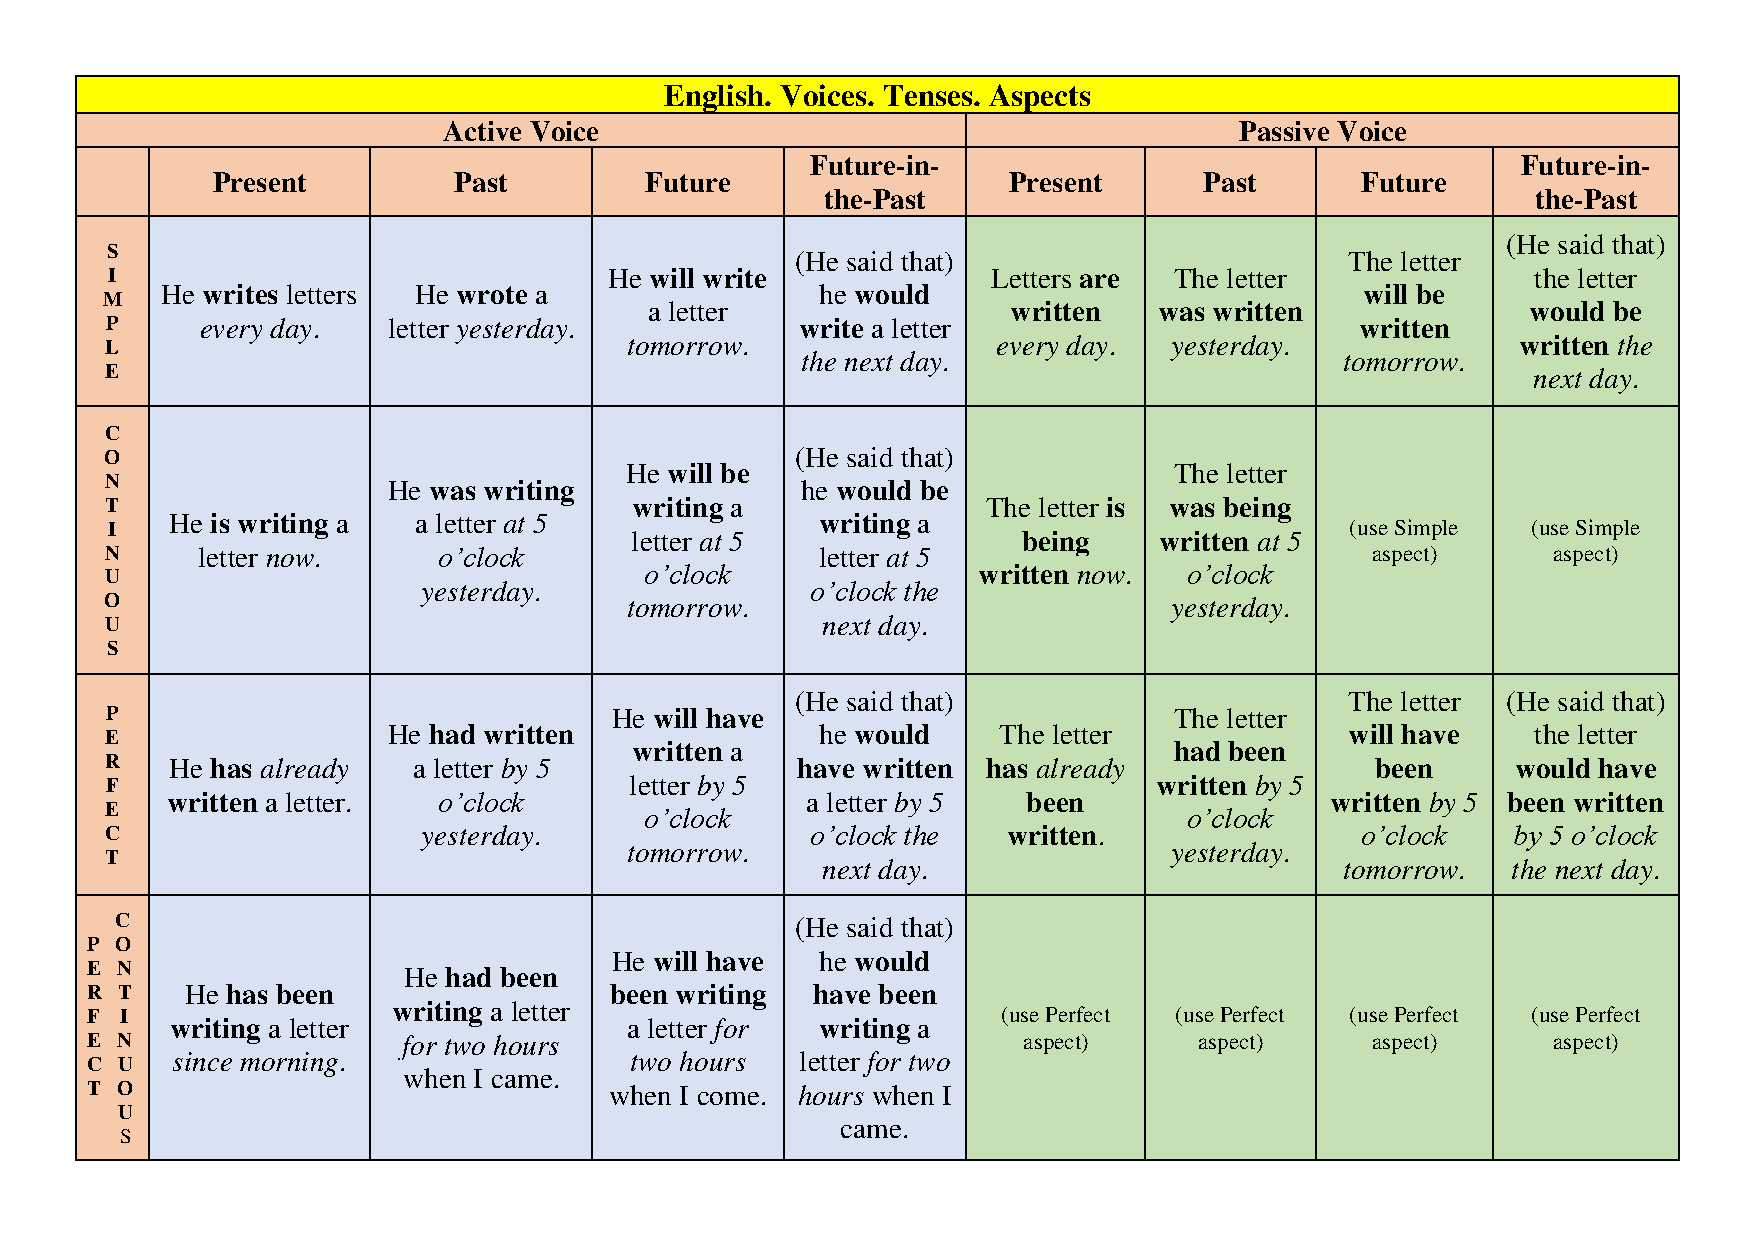
\includegraphics[angle=90,width=\textwidth,page=1,trim={0.5in 0.2in 0.49in 0.2in},clip=true]{EnglishTensesAspectsVoicesPoster.pdf}}

\end{document}
